\newpage

\section{Resultados}
\subsection{Conversor digital-análogo}

\begin{verbatim}
RESET:
    ; Apuntar Z al inicio de la LUT
    ldi ZH, HIGH(LUT_START<<1)
    ldi ZL, LOW(LUT_START<<1)

    ; Apuntar Y al final de la LUT
    ldi YH, HIGH(LUT_END<<1)
    ldi YL, LOW(LUT_END<<1)
\end{verbatim}

\begin{verbatim}
MAIN_LOOP:
    ; Leer siguiente valor de la LUT
    ; y avanzar puntero
    lpm r16, Z+
    out PORTD, r16
    rcall delay

    cp  ZL, YL
    cpc ZH, YH
    ; Si no es el fin, seguir
    brne MAIN_LOOP

    ; Volver al inicio de la tabla
    ldi ZH, HIGH(LUT_START<<1)
    ldi ZL, LOW(LUT_START<<1)
    rjmp MAIN_LOOP
\end{verbatim}

\begin{figure}[H]
  \centering
  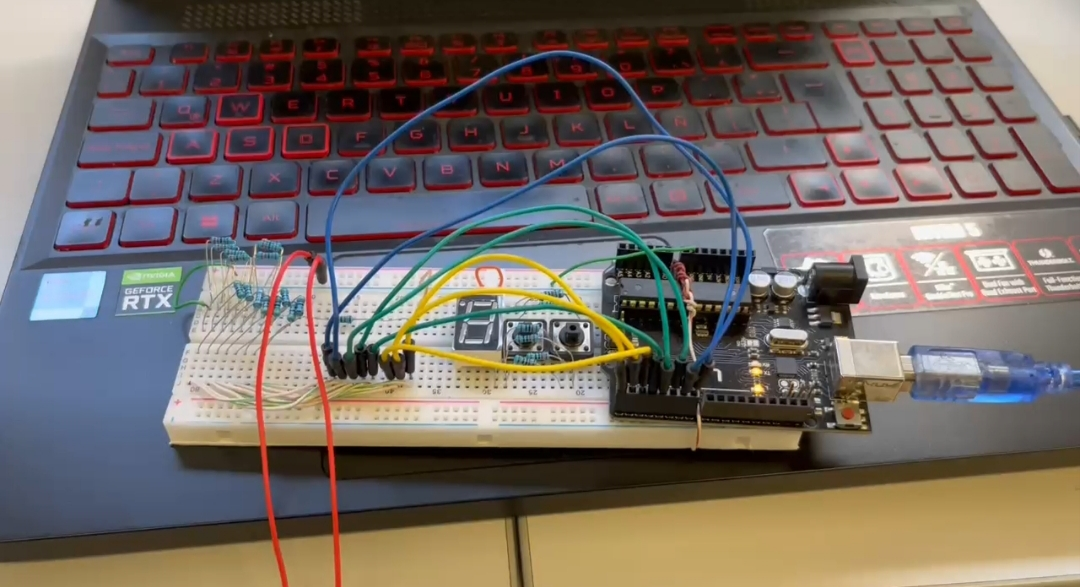
\includegraphics[width=\linewidth]{./Anexos/Resultados/DAC/Circuito.jpg}
  \caption{Circuito final para conversor digital-análogo. Fuente: \cite{LabDrive}.}
  \label{fig:conversor_circuito}
\end{figure}

\begin{figure}[H]
  \centering
  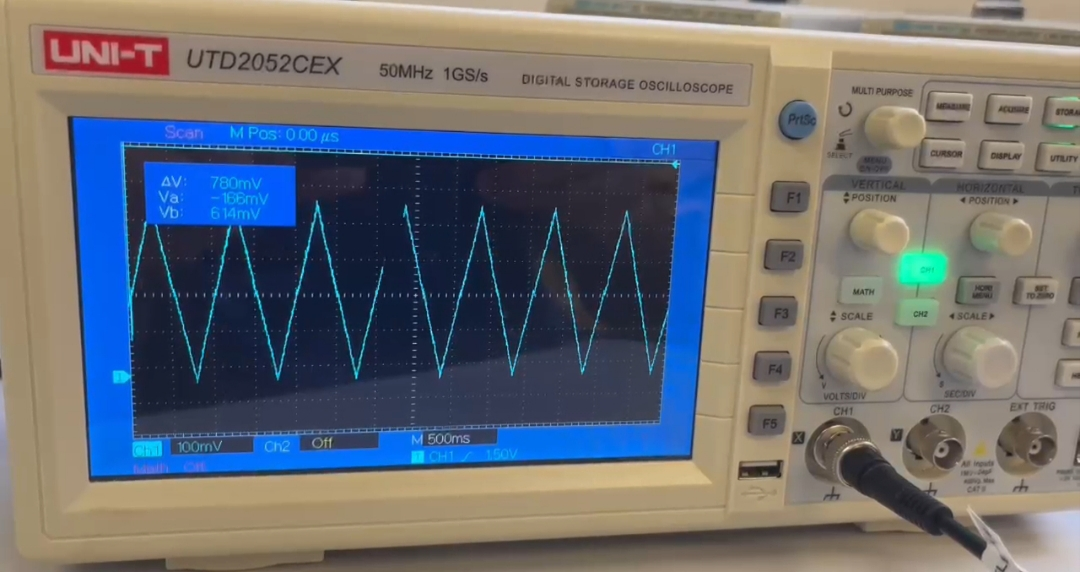
\includegraphics[width=\linewidth]{./Anexos/Resultados/DAC/Ocsiloscopio.jpg}
  \caption{visualización de señal en osciloscopio. Fuente: \cite{LabDrive}.}
  \label{fig:conversor_osciloscopio}
\end{figure}

\subsection{Matriz}

\subsubsection{Mapeado de puertos y pines}
Se mapean los puertos y pines individuales del mismo modo al que se puede apreciar en el anexo \ref{anexo:Look_Up_Table}. 

\subsubsection{Encendido de un solo LED}
Utilizando la LUT, se recorre añadiendo la posición especificada previamente en los registros \texttt{row} y \texttt{col}, para encender especificamente el LED mapeado a esa fila y columna. La función hace uso de \texttt{CLEAR\_LED} y \texttt{SET\_LED} (Véase anexo \ref{anexo:Bit_Masks}) para encender la fila y columna respectivamente, sin modificar el resto de bits en los puertos. 

\begin{verbatim}
ldi ZH, high(ROW_PORTS<<1) 
ldi ZL, low(ROW_PORTS<<1)
add ZL, row adc ZH, r1  
lpm r16, Z ; r16 = row port adress
        
ldi ZH, high(ROW_MASKS<<1) 
ldi ZL, low(ROW_MASKS<<1)
add ZL, row adc ZH, r1
lpm r17, Z ; r18 = row pin mask

; Encender fila
clr ZH mov ZL, r16 
mov r16, r17
rcall CLEAR_BIT

ldi ZH, high(COL_PORTS<<1) 
ldi ZL, low(COL_PORTS<<1)  
add ZL, col adc ZH, r1  
lpm r16, Z ; r16 = column port adress

ldi ZH, high(COL_MASKS<<1) 
ldi ZL, low(COL_MASKS<<1)  
add ZL, col adc ZH, r1  
lpm r17, Z ; r17 = column pin mask

; Encender columna
clr ZH mov ZL, r16 
mov r16, r17
rcall SET_BIT
\end{verbatim}

\subsubsection{Multiplexado y dibujo de cuadros}
Al encender un LED solo muy rápido se realizan operaciones condicionales con una máscara guardada en FLASH que representa la imágen del fotograma. Cada LED individual es comparado utilizando \texttt{r16}, el cual guarda la máscara posicional con la cual se realiza una operación \texttt{AND} para identificar si el LED se prendería en ese fotograma o no. 

\begin{verbatim}
ldi row, 0 RENDER_FRAME_ROW_LOOP:  
ldi r16, 0b00000001 ; Frame mask
lpm r17, Z+

ldi col, 0 RENDER_FRAME_COL_LOOP:
    rcall CLEAR_MATRIX

    push r16
    and r16, r17

    cpi r16, 0 
    breq RENDER_FRAME_SKIP_LED

    rcall TURN_LED
    rcall TEST_DELAY

    RENDER_FRAME_SKIP_LED:
    pop r16
    lsl r16
inc col cpi col, 8 
brlo RENDER_FRAME_COL_LOOP 

inc row cpi row, 8 
brlo RENDER_FRAME_ROW_LOOP
\end{verbatim}

\subsubsection{USART}
Utilizando la interrupción de overflow del \texttt{TIMER2} configurada para 100ms, se pueden realizar animaciones de texto desplazante, por ejemplo, al incrementar la posición del puntero del fotograma actual dentro de la misma interrupción. Utilizando lógica de estados Y USART asíncrono con un buffer de anillo (véase anexo \ref{anexo:USART_Asincrono_con_Ring_Buffer}), se programan las diferentes funcionalidades menú de inicio, mostrar un texto desplazante o mostrar difernetes imágenes en la matriz (véase anexo \ref{anexo:Maquina_de_Estados}).


\begin{figure}[H]
  \centering
  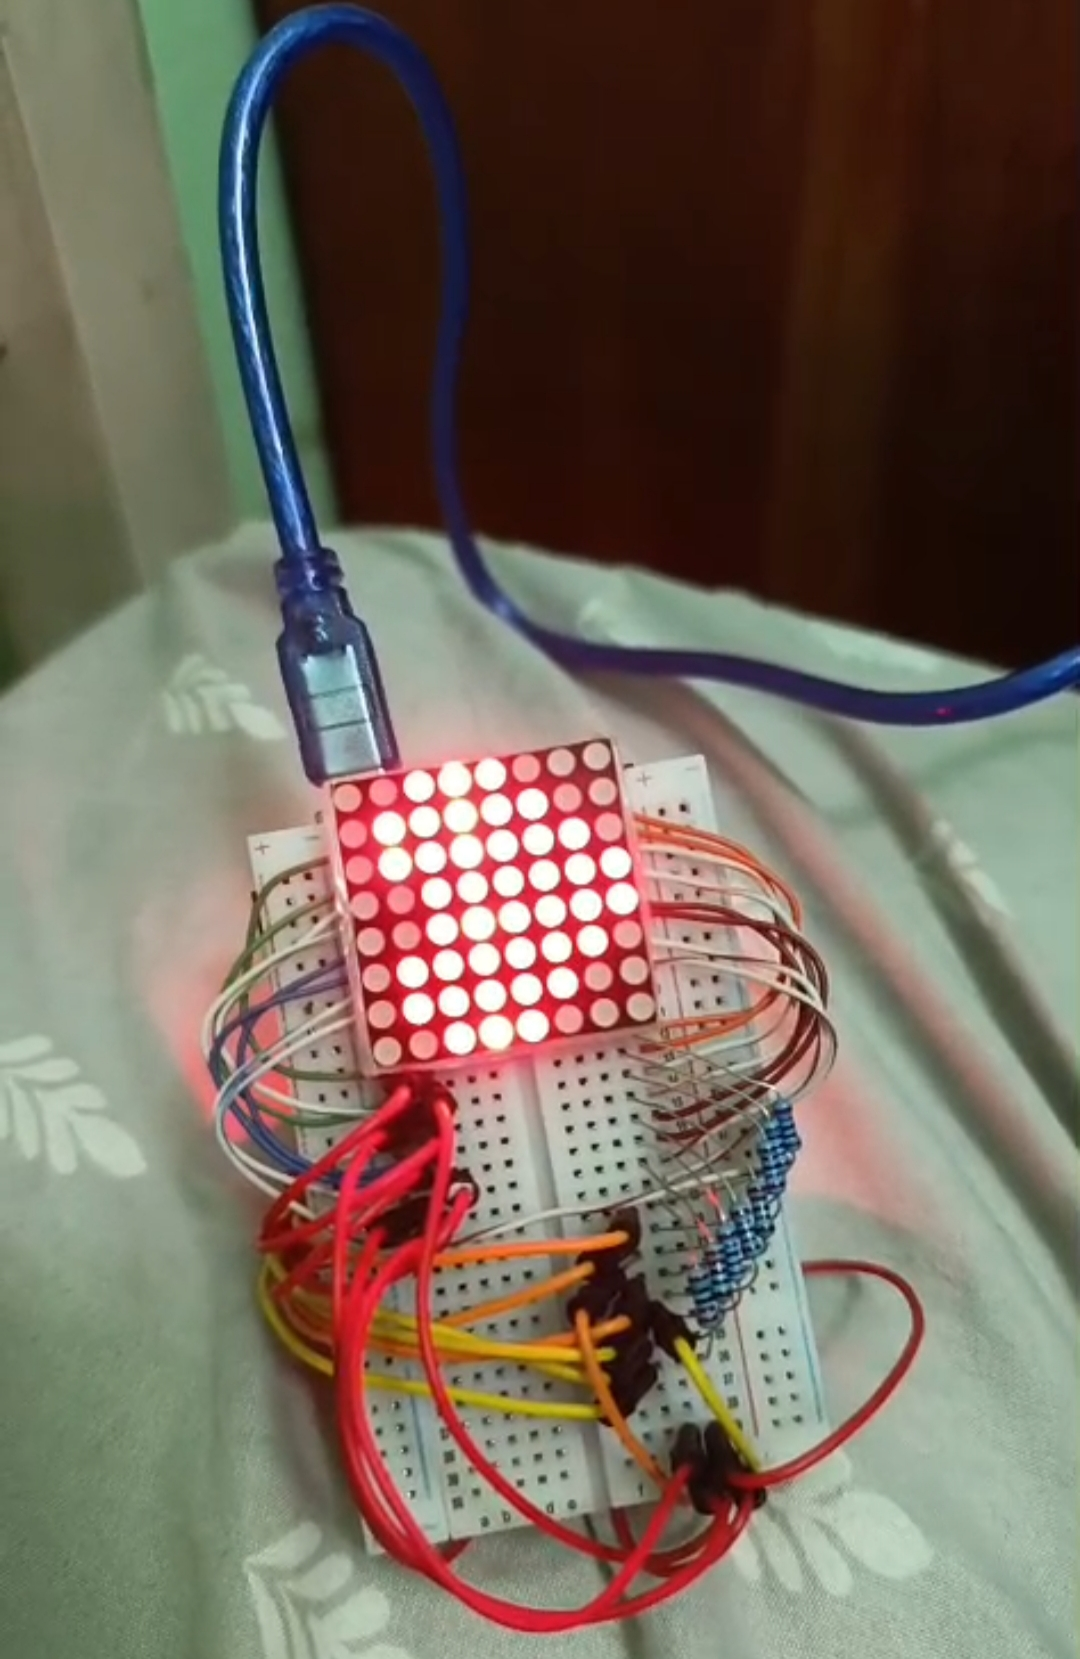
\includegraphics[width=0.7\linewidth]{./Anexos/Resultados/Matriz/Circuito.jpg}
  \caption{Circuito final para Matriz de LEDs. Fuente: \cite{LabDrive}.}
  \label{fig:circuito_matriz}
\end{figure}

\begin{figure}[H]
  \centering
  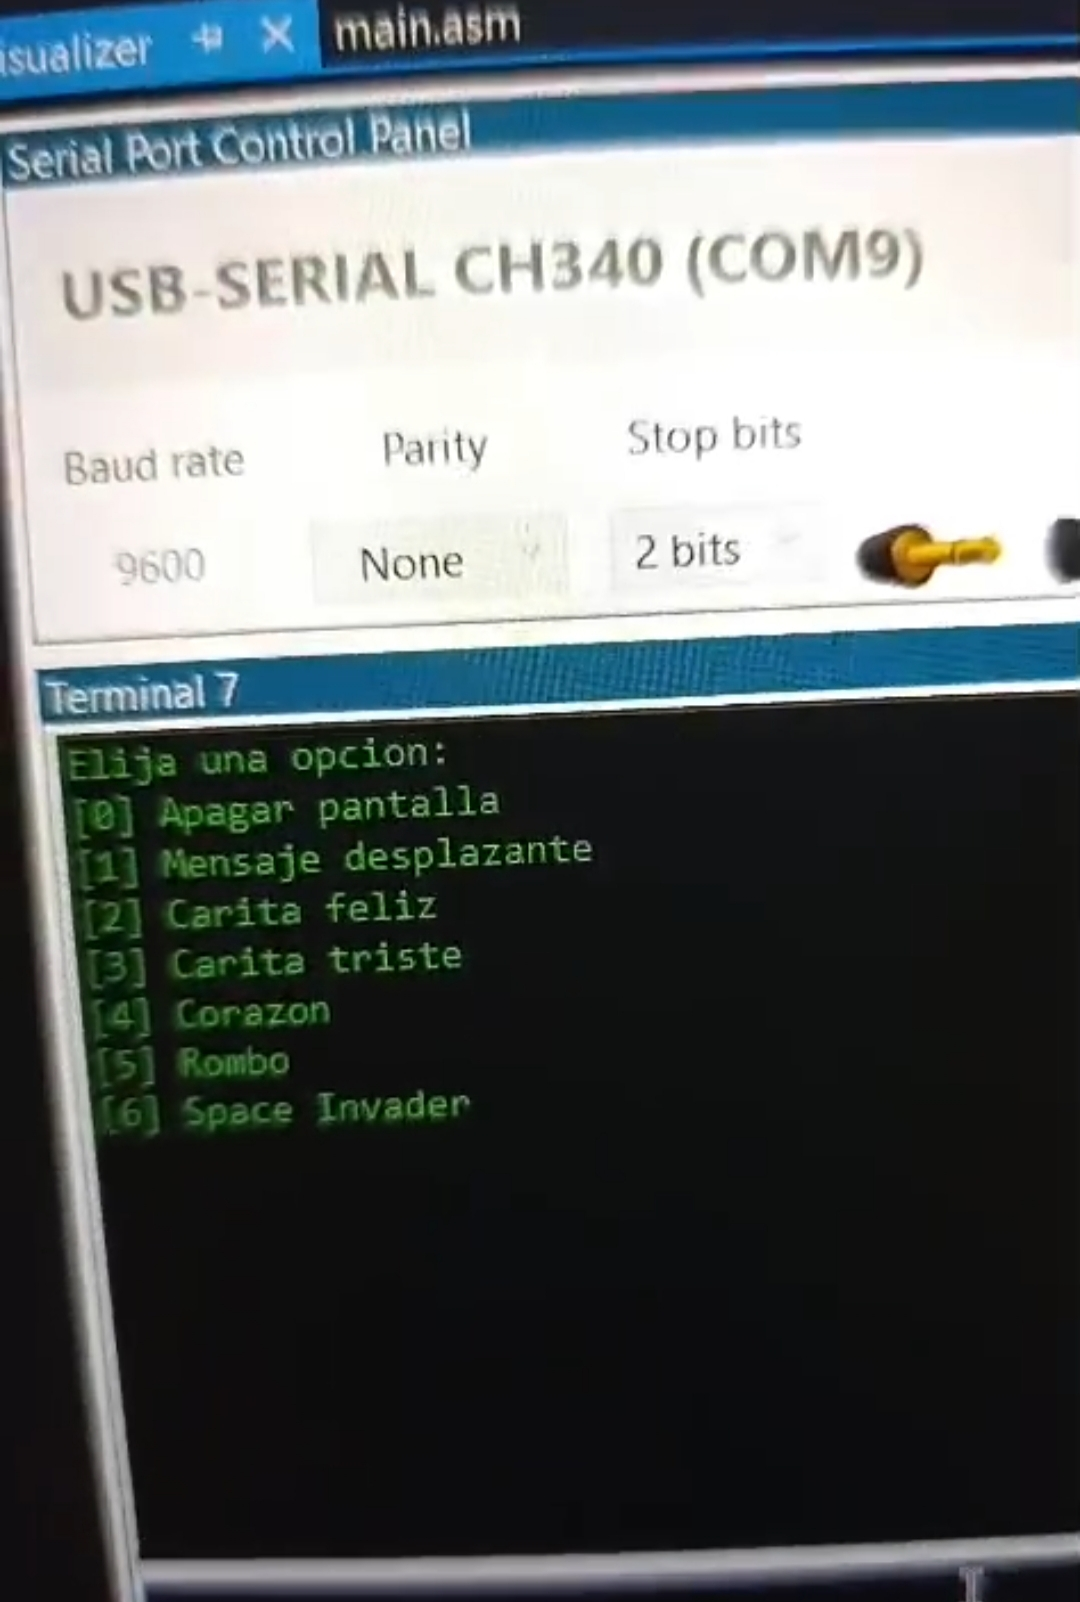
\includegraphics[width=0.7\linewidth]{./Anexos/Resultados/Matriz/Menu.jpg}
  \caption{Menu de opciones para Matriz de LEDs. Fuente: \cite{LabDrive}.}
  \label{fig:menu_matriz}
\end{figure}



\subsection{Punzonadora}

\subsubsection{Configuración de temporizador variable}
Se utilizan macros para realizar el control de temporizadores. En este caso se muestra como se configura al \text{TIMER1} para realizar una determinada cantidad de overflows de 1 segundo cada uno. 

\begin{verbatim}
.macro ENABLE_TIMER_1
; @0 Timer seconds
push r16
mov timer1_ovf_counter, @0
ldi r16, 0b101		 sts TCCR1B, r16
ldi r16, HIGH(49911) sts TCNT1H, r16
ldi r16, LOW(49911)	 sts TCNT1L, r16 
ldi r16, (1<<TOV1)   out TIFR1,  r16 
ldi r16, (1<<TOIE1)  sts TIMSK1, r16 
pop r16
.endmacro
\end{verbatim}


\subsubsection{Manejo de estados}
El manejo de estados del sistema es una máquina de estados como la que se puede ver en el anexo \ref{anexo:Maquina_de_Estados}. Aquí se muestra un fragmento con los estados internos:

Control de estados general:
\begin{verbatim}
STATE_MACHINE:
cpi state, 0 breq STATE_MACHINE_STOP
cpi state, 1 breq STATE_MACHINE_ADVANCE
cpi state, 2 breq STATE_MACHINE_WAIT_1
cpi state, 3 breq STATE_MACHINE_PUNCH
cpi state, 4 breq STATE_MACHINE_WAIT_2
cpi state, 5 breq STATE_MACHINE_EXTRACT
rjmp STATE_MACHINE_END
\end{verbatim}

Luego en cada estado individual existe una serie de condicionales que determinará el tiempo con el que se confgiura \texttt{TIMER1} para pasar al siguiente estado, dependiendo de la carga configurada.
\begin{verbatim}
STATE_MACHINE_STOP:
cpi load, 0 breq STOP_LOAD_0
cpi load, 1 breq STOP_LOAD_1
cpi load, 2 breq STOP_LOAD_2
rjmp STATE_MACHINE_STOP_SKIP
\end{verbatim}

\subsubsection{Botones, LEDs,  y debouncing}
En Standby se enciende el indicador izquierdo verde, indicando que el sistema está esperando la señal de arranque, ya sea por USART o por los pulsadores físicos. Con el pulsador de la izquierda se maneja el cambio de carga, el cual hace un ciclo de cambio entre liviana, mediana, y pesada, indicadas por LEDs de color verde, amarillo, y rojo, respectivamente.

En este fragmento de código se muestra como se maneja de deobuncing, y pausado de entradas externas durante el funcionamiento de la máquina: cuando esta arranca su funcionamiento se desabilitan las interrupcioens externas, y las interrupciones de recepción de USART. Se vuelven a habilitar una vez la máquina de estados reconoce que llegó al final de la secuencia. Se implementaron macros para la habilitación y deshabilitación de interrupciones.

\begin{verbatim}
INT0_ISR:
    push r16
    in r16, SREG
    push r16 

    DISABLE_BUTTONS
    DISABLE_RX

    ldi state, 1
    ldi r16, 1 
    sts event_pending, r16

    pop r16
    out SREG, r16
    pop r16 
    reti
\end{verbatim}

Temporizador de deboucing para botones de cambio de carga. Timer 2 configurado para un overflow de aproximadamente 1 segundo (usando contador de overflow externo):

\begin{verbatim}
    T2_OVF_ISR:
	push r16 
    in r16, SREG 
	push r16 
	
	inc timer2_ovf_counter
	
	ldi r16, _TIMER2_OVF_COUNT 
    cp r16, timer2_ovf_counter 
    brsh T2_OVF_ISR_END 
    
	DISABLE_TIMER_2
	ENABLE_BUTTONS
	clr timer2_ovf_counter
    
    T2_OVF_ISR_END:
		pop r16
		out SREG, r16
		pop r16	
		reti

\end{verbatim}


\subsubsection{USART}
Identico para los otros casos, se configura un menú que es enviado en el RESET del programa para ser mostrado al inicio, y una serie de condicionales determinan el comportamiento del sistema dependiendo del comando que recibe. En este caso: 1, 2, y 3 para seleccionar el tipo de carga. Y A para iniciar la secuencia del programa.


\begin{figure}[H]
  \centering
  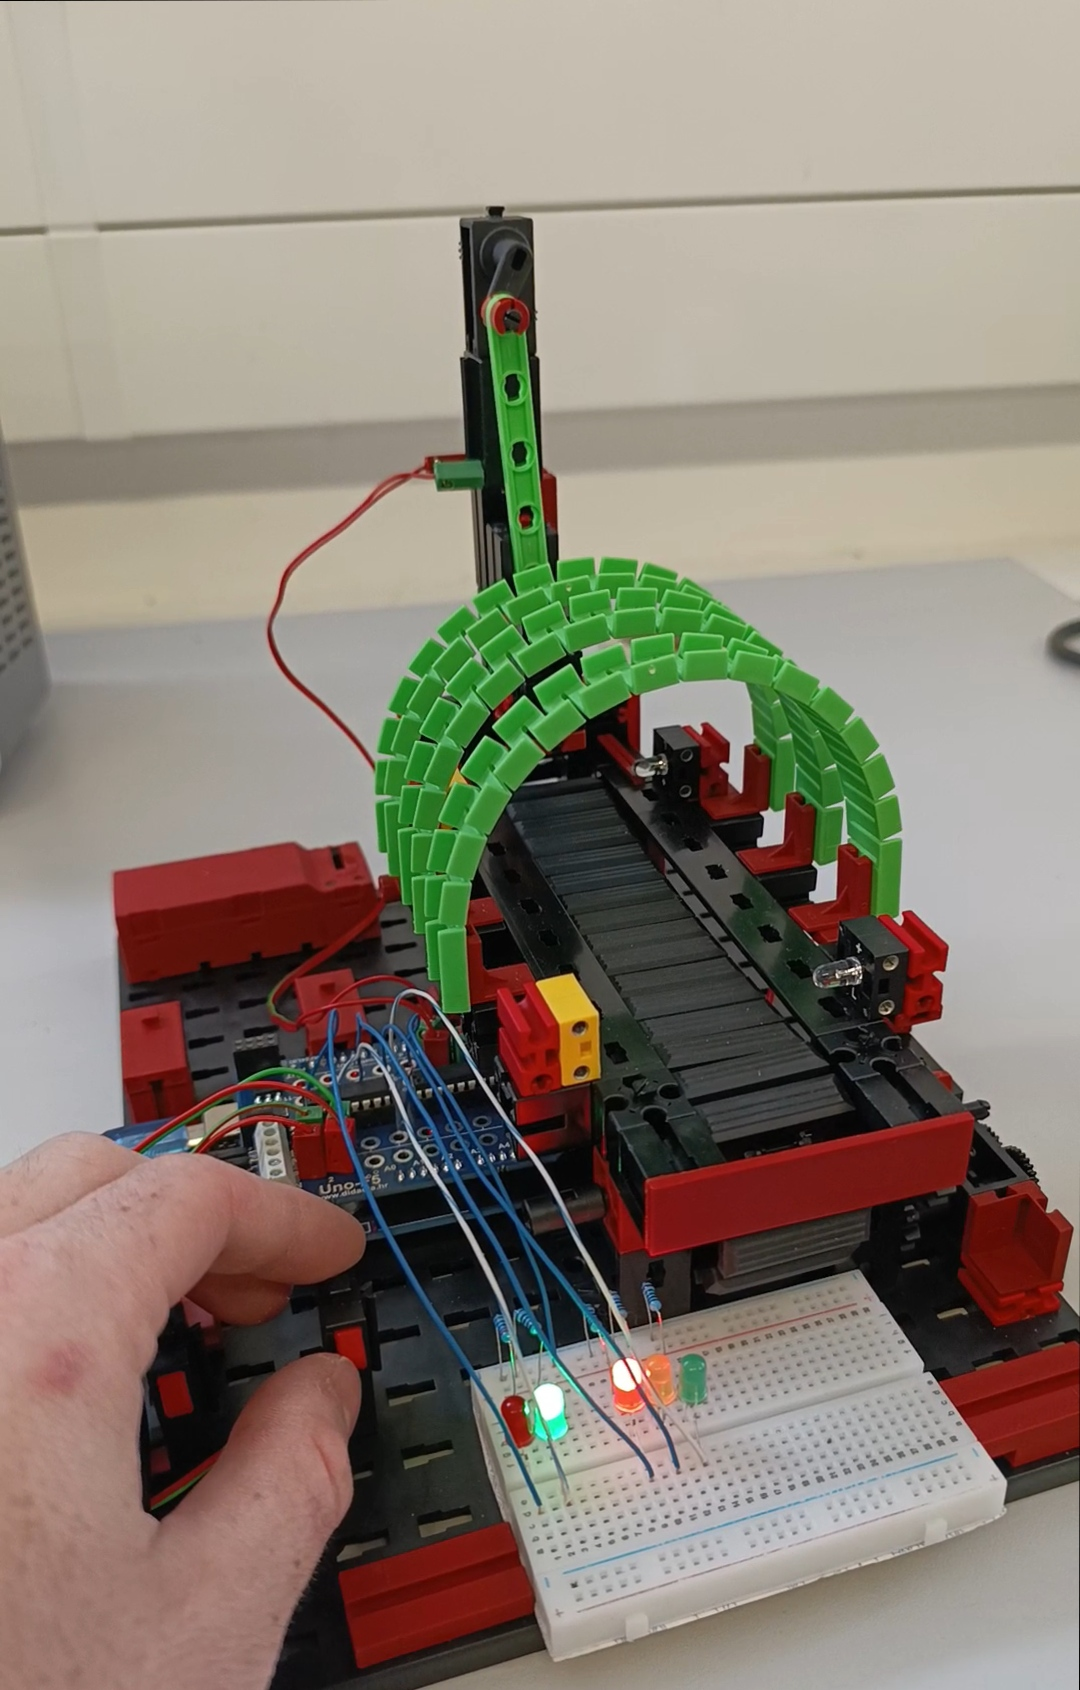
\includegraphics[width=0.7\linewidth]{./Anexos/Resultados/Punzonadora/Circuito.jpg}
  \caption{Ensamblado final de punzonadora. Fuente: \cite{LabDrive}.}
  \label{fig:punzonadora_circuito}
\end{figure}

\subsection{Plotter}

Utilizando \texttt{.equ} se mapean las instrucciones de la tabla a un nombre fácil de interpretar. La ventaja que se tiene al tratarse de bits individuales, es que luego se podrán realizar operaciones como \texttt{UP + RIGHT} para comandar al plotter el movimeinto arriba a la derecha de manera más legible e intuitiva.

\subsubsection{Mapeo de comandos}
\begin{verbatim}
.equ SOLENOID_DOWN =  0b00000100
.equ SOLENOID_UP   =  0b00001000
.equ DOWN          =  0b00010000
.equ UP            =  0b00100000
.equ RIGHT         =  0b01000000
.equ LEFT          =  0b10000000
.equ STOP          =  0b00000000
\end{verbatim}

El siguiente ejemplo es de un programa hecho para el interprete creado para el plotter:
\begin{verbatim}
TRIANGLE_DATA:
    .db 5,  SOLENOID_DOWN	
    .db 20, SOLENOID_DOWN + RIGHT			
    .db 10, SOLENOID_DOWN + UP + LEFT		
    .db 10, SOLENOID_DOWN + DOWN + LEFT
    .db 5,  SOLENOID_UP		
    .db 5,  STOP
\end{verbatim}

\subsubsection{Interprete de secuencias programadas}

El interprete \texttt{DRAW} se encarga de escribir el valor guardado en la secuencia en \texttt{PORTD}, y esperar la cantidad de tiempo indicada en la misma antes de pasar a la siguiente instrucción.

\begin{verbatim}
DRAW:
    mov ZL, r16 mov ZH, r17
    DRAW_LOOP:
    lpm r18, Z+ ; Time
    lpm r19, Z+ ; Instruction

    out PORTD, r19 ; Send instruction

    cpi r19, STOP
    breq DRAW_END ; Stop drawing

    DRAW_TIMER_LOOP: 
    rcall S1 ; Timer
    dec r18 brne DRAW_TIMER_LOOP 

    rjmp DRAW_LOOP ; Next instruction

    DRAW_END:
    ret
\end{verbatim}
Se encontró que para temporizadores con valores menores a 1ms no permitían el movimiento adecuado de los motores, por lo cual se decidió limitar la resolución con un temporizador de 1500 $\mu S$

\subsubsection{USART}
Luego se utiliza la funcionalidad de USART asíncrono con Ring Buffer mostrada en el anexo \ref{anexo:USART_Asincrono_con_Ring_Buffer}, para mostrar un menú en el inicio del programa y darle la opción al usuario de elegir entre diferentes comandos para el plotter. Se agregaron las funcionalidades \texttt{ARRIBA, ABAJO, IZQUIERDA, DERECHA} para permitir posicionar el solenoide del plotter antes de realizar el trazado de las figuras.

\begin{figure}[H]
  \centering
  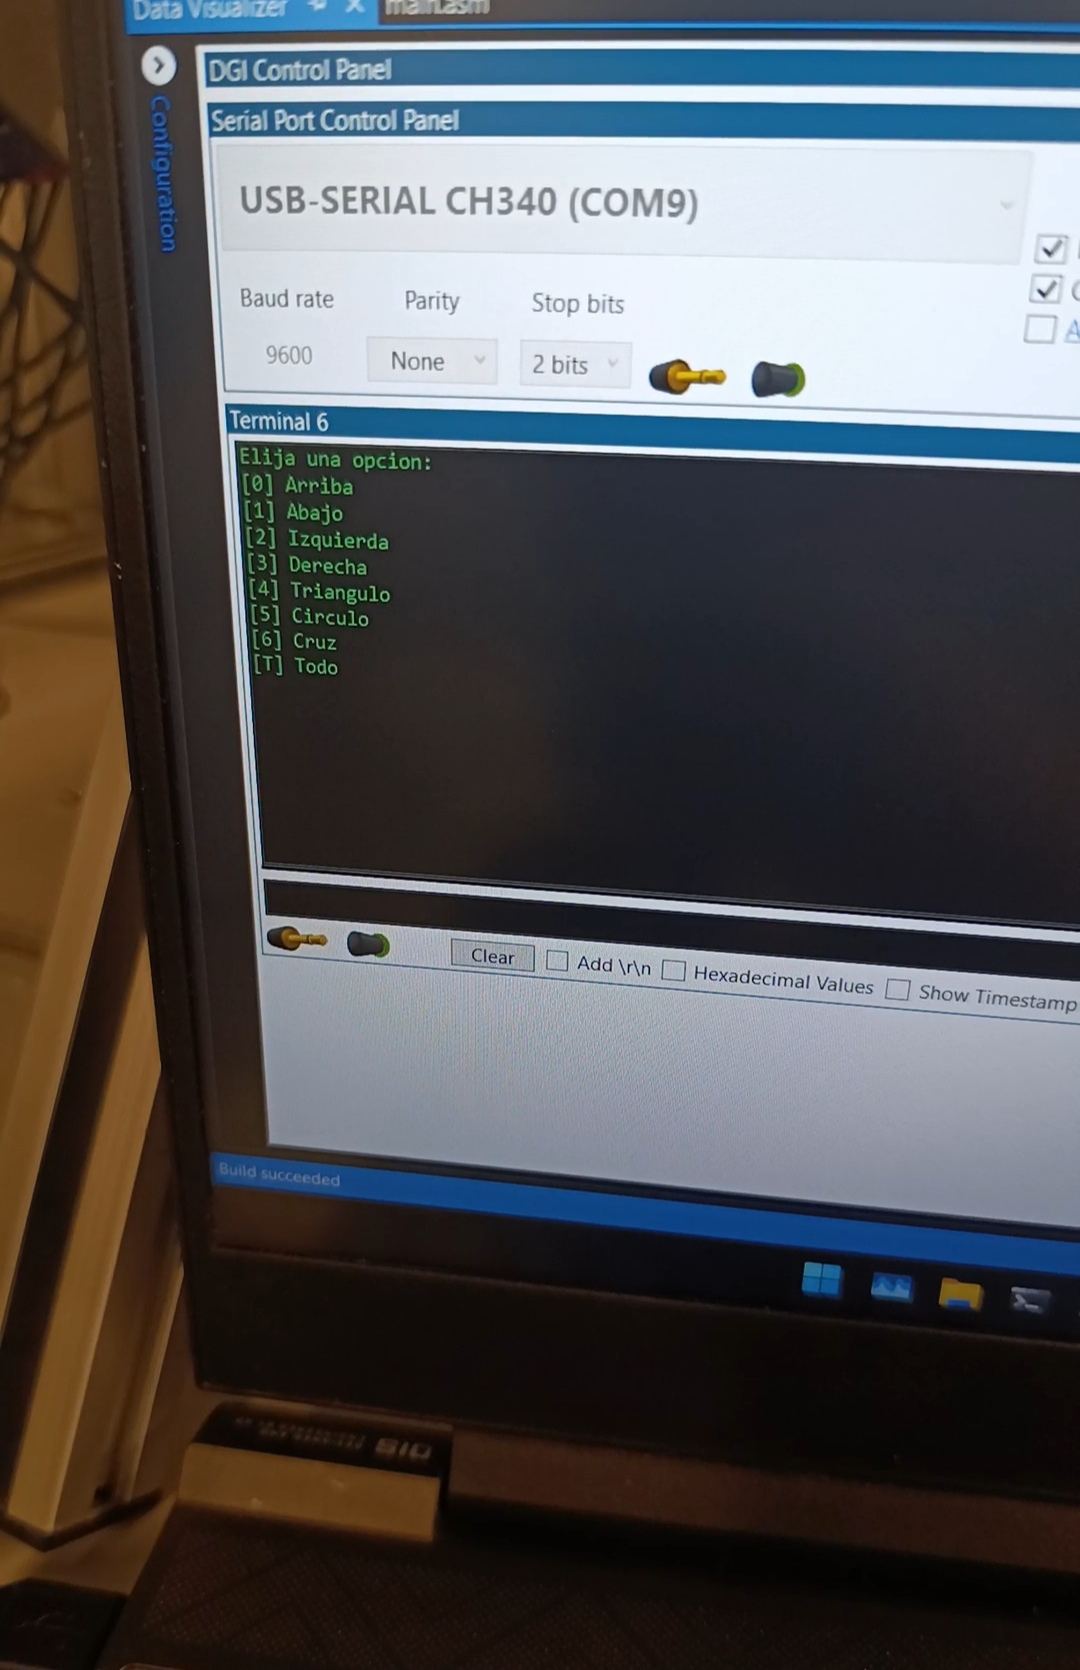
\includegraphics[width=0.7\linewidth]{./Anexos/Resultados/Plotter/Menu.jpg}
  \caption{Menu en USART para el Plotter. Fuente: \cite{LabDrive}.}
  \label{fig:plotter_menu}
\end{figure}

\begin{figure}[H]
  \centering
  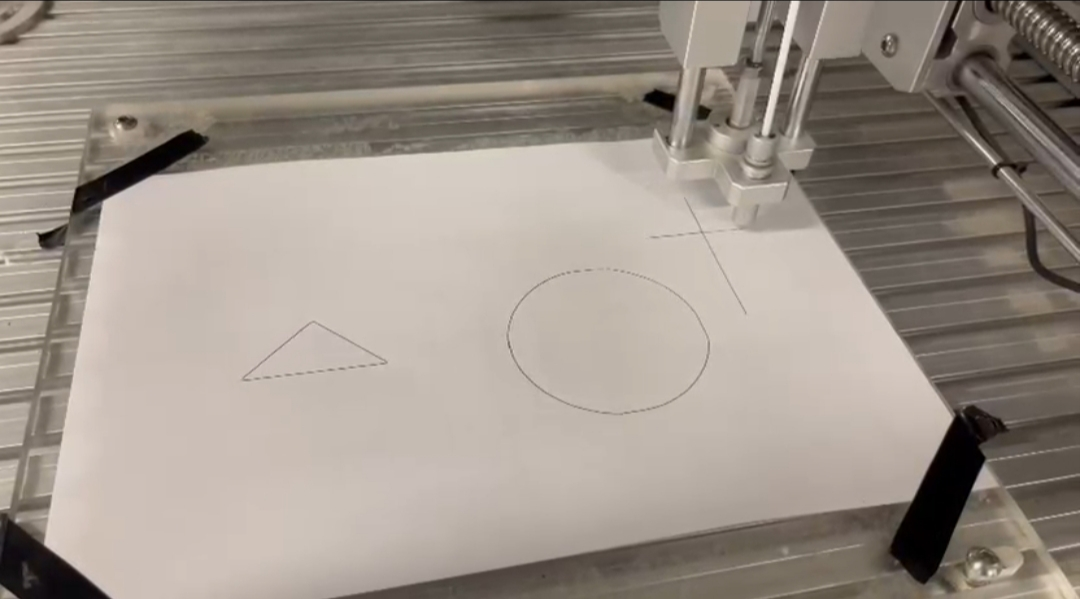
\includegraphics[width=\linewidth]{./Anexos/Resultados/Plotter/Dibujos.jpg}
  \caption{Figuras dibujadas en el plotter. Fuente: \cite{LabDrive}.}
  \label{fig:plotter_figuras}
\end{figure}